\chapter{Samplers and the Horizon}\label{chap:samplers}

\Cref{chap:computation} asked what computation can prove. This chapter asks what
simulation can find. The idea, suggested by the Bayesian computation
literature, is to treat the problem as one of rare event simulation. Define an energy on
the integers, say the total stopping time, declare the integers with high energy to
be the interesting ones, and use a sampler that climbs the energy landscape to
find them or to measure how many there are. Nested sampling\index{nested sampling}, the vertical
likelihood\index{vertical likelihood} sampler and split sampling\index{split sampling} are three such methods, all built to
estimate a normalizing constant by moving through a sequence of level sets
rather than by sampling the base measure directly, and, given exact draws from each level set, all three
reach regions of exponentially small prior mass in a number of steps that is
polynomial in the depth. The question this chapter answers is whether such a
method can say anything about the conjecture in polynomial time. It can do one
thing exactly, which we prove, and beyond a horizon a local sampler leaves the tree of merged orbits it starts in only about as often as rejection sampling finds a new one, which we explain heuristically in the Bernoulli model and observe in practice.

\section{One identity, three samplers}

Let $\pi$ be a probability measure on a space $\mathcal X$ and let
$L:\mathcal X\to[0,\infty]$ be an energy. Write
\[
  Z(m)=\pi\{L>m\},\qquad m\ge0,
\]
for the prior volume of the level set\index{level set} above $m$. The quantity every method
estimates is the expected energy, or more generally $\E_\pi[g(L)]$ for a
monotone $g$, through the layer cake identity
\begin{equation}\label{eq:ch10b:cake}
  \E_\pi[L]=\int_0^\infty Z(m)\,dm .
\end{equation}
The common device is a level variable. Fix a weight, a measure $\omega$ on $[0,\infty)$ with cumulative weight $W(l)=\omega([0,l))$ finite for every $l$, and consider the joint law
\begin{equation}\label{eq:ch10b:aug}
  \pi_\omega(dx,dm)\ \propto\ [\,L(x)>m\,]\,\pi(dx)\,\omega(dm) ,
\end{equation}
which is a probability law when its total mass $\int Z\,d\omega=\E_\pi[W(L)]$ is finite.
Its two marginals are read off at once: integrating out $m$ gives $x$ the law
proportional to $W(L(x))\pi(dx)$, and integrating out $x$ gives $m$ the law
proportional to $Z(m)\,\omega(dm)$. Polson\index{Polson, N. G.} and Scott\index{Scott, J. G.}~\cite{polsonscott2015} call a
Markov chain that alternates the two conditionals, $m$ given $x$ and $x$ given
$m$, a weighted slice sampler\index{slice sampling}, and show that vertical likelihood and nested sampling are choices of the weight; Birge\index{Birge, J. R.}, Chang\index{Chang, C.} and Polson~\cite{birge2013} show the same for split sampling.

\begin{enumerate}[label=(\roman*),leftmargin=2em]
\item \emph{Vertical likelihood.} Take the cumulative weight $W=1/Z$, that is a unit atom at $m=0$ together with the density $(1/Z)'$. The level marginal is then proportional to $-Z'(m)/Z(m)$ away from $0$, which is flat in the coordinate $\log(1/Z(m))$: the chain spends equal time in each factor $e$ of prior volume, and the $x$ marginal is $\pi$ reweighted by $W(L(x))=1/Z(L(x))$, which grows like $e^{DL}$ when $Z(m)\approx e^{-Dm}$. With this weight the augmented law has infinite mass when $L$ is continuous, since $Z(L)$ is then uniform on $(0,1)$, and Polson and Scott floor the weight, $W(m)=1/\max(\eta,Z(m))$, to keep the law proper~\cite[eq.~(19)]{polsonscott2015}. Since $Z$ is unknown one uses a running estimate $\hat Z$ in its place, and recovers $Z(m)$ from the chain by importance weighting each sample $x$ with $1/W(L(x))$.
  The conditional of $m$ given $x$
  is explicit: draw $T$ uniform on $(0,1/\max(\eta,Z(L(x))))$ and set $m=0$ if
  $T\le1$ and $m=Z^{-1}(1/T)$ otherwise~\cite[Lemma 3]{polsonscott2015}.
\item \emph{Nested sampling.} Skilling\index{Skilling, J.}~\cite{skilling2006} discretizes the
  same weight $W=1/Z$. A population of $N$ live points is drawn from
  $\pi$; at each iteration the point of lowest energy $L_i$ is removed and
  replaced by a draw from $\pi$ conditioned on $\{L>L_i\}$, obtained by running
  a $\pi$ invariant Markov kernel inside the level set. The prior volume above
  $L_i$ shrinks by a factor with mean $N/(N+1)\approx e^{-1/N}$, whose logarithm has mean exactly $-1/N$, per iteration,
  which is the flat level marginal in logarithmic coordinates, and
  \eqref{eq:ch10b:cake} is estimated by the quadrature
  $\sum_i(X_{i-1}-X_i)\,g(L_i)$ with $X_i=e^{-i/N}$.
\item \emph{Split sampling.} Birge, Chang and Polson~\cite{birge2013} fix the
  levels adaptively at quantiles instead: at stage $t$ the sampler runs inside
  $\{L>m_{t-1}\}$, sets $m_t$ to the $(1-\rho)$ quantile of the energies it
  sees, and records the conditional fraction $p_t\approx\rho$ above $m_t$. The
  product $\prod_{s\le t}p_s$ estimates $Z(m_t)$; this is the product estimator, which they show is split sampling with the discrete weights $\omega_t=1/Z(m_t)$ (their Theorem~1).
  If the stage estimates are independent with relative variances $v_t$, the relative variance of the product is $\prod_t(1+v_t)-1$; with $N$ independent samples per stage $v_t\approx(1-\rho)/(\rho N)$, and the product is about $t(1-\rho)/(\rho N)$, linear in the number of stages $t=\log(1/Z)/\log(1/\rho)$, when $N$ is large compared with $t$.
  The Rao
  Blackwellized estimate
  $\hat Z(m)=\sum_{x:L(x)>m}\Omega(L(x))^{-1}\big/\sum_x\Omega(L(x))^{-1}$,
  with $\Omega=W$ the cumulative weight actually used, recovers the whole curve $Z$ from
  one run; with $\Omega=1/Z$ the sampling distribution of the method matches that of nested sampling, which
  is their Theorem~2.
\end{enumerate}

In every case the work per sample is polynomial in the depth, provided one
ingredient: a kernel that moves freely inside each level set $\{L>m\}$. The
cost of a method is the cost of that kernel, and the obstruction we will meet
is that for the natural Collatz energy no local kernel moves freely at depth.

\section{The Collatz prior and two energies}

The only natural prior on the integers is the one the $2$ adic formulation
provides, the Haar measure $\mu$ on $\Ztwo$ of \cref{chap:parity}, under which
the residue modulo $2^k$ is uniform for every $k$ and the parity digits of the
orbit are independent fair coins (\cref{thm:terras}). Two energies suggest
themselves. The first is the coefficient stopping time $\tau$ of \cref{def:ch2:stopping}, the
first $k$ at which $3^{m_k}<2^k$, which is a function of the parity word of
length $k$ and so of the residue class modulo $2^k$. The second is the total
stopping time\index{stopping time} $\sigma_\infty$, the first $k$ with $T^{(k)}(n)=1$, counted in steps of $T$ (in \cref{chap:intro} the same symbol counts steps of $T_0$), which is the
quantity the conjecture is about. The two are separated by a horizon.

\begin{proposition}[Two energies]\label{prop:ch10b:horizons}
\leavevmode
\begin{enumerate}[label=(\roman*),leftmargin=2em]
\item For every $m$ the level set $\{\tau>m\}\subset\Ztwo$ is a union of
  residue classes modulo $2^m$, hence open and closed, and its Haar measure is
  $Z_\tau(m)=1-F(m)=2^{-m}\sum_jN_m(j)$, computable exactly in $O(m^2)$
  arithmetic operations by \cref{prop:ch2:dp}. The sets decrease in $m$ and
  their intersection $\{\tau=\infty\}$ has measure zero.
\item For every $m$ the set $\{x\in\Ztwo:\sigma_\infty(x)\le m\}$ is finite, and it contains at most one positive integer in each residue class modulo $2^m$.
  Consequently $\{\sigma_\infty>m\}$ has Haar measure one for every $m$, and so does the intersection $\{\sigma_\infty=\infty\}$ of these sets: the energy $\sigma_\infty$ is almost surely infinite under $\mu$, and any simulation with this energy must use a uniform prior on a finite range, which we take to be $[2,2^B)$, with $Z_\sigma(m)=\#\{2\le n<2^B:\sigma_\infty(n)>m\}/(2^B-2)$.
\end{enumerate}
\end{proposition}

\begin{proof}
(i) is the content of \cref{sec:ch2:terras} and \cref{prop:ch2:dp}: $\tau(n)>m$
is decided by the first $m$ parities, which are a bijective function of
$n\bmod2^m$, and the density theorem of \cref{chap:parity} says
$1-F(m)\to0$.
For (ii), every $y\in\Ztwo$ has exactly the two preimages $2y$ and $(2y-1)/3$ under $T$, so $\{\sigma_\infty\le m\}$, which lies in $\bigcup_{k\le m}T^{-k}(1)$, has at most $2^{m+1}-1$ points.
Now fix a parity word $w$ of length $m$ with $j$ ones. By the Terras formula $T^{(m)}(n)=(3^jn+c_w)/2^m$ for every $n$ in the class of $w$, and $\sigma_\infty(n)\le m$ forces $T^{(m)}(n)\in\{1,2\}$, because the orbit alternates between $1$ and $2$ once it reaches $1$; so $n=(2^m-c_w)/3^j$ or $n=(2^{m+1}-c_w)/3^j$.
These differ by $2^m/3^j$, so both are integers only when $j=0$; then $w$ is the zero word, $c_w=0$, and of $2^m$ and $2^{m+1}$ only the first has $\sigma_\infty\le m$.
Hence each class contains at most one positive integer with $\sigma_\infty\le m$, the complement of a finite set has full Haar measure, and so does a countable intersection of such complements.
\end{proof}

The horizon is the following. The event $\{\tau>m\}$ reads only the first $m$ parities, which are a bijective function of the residue modulo $2^m$, so its level sets have the clopen
structure a sampler needs: a residue class is a cylinder, and moving inside a
union of cylinders is easy. An integer below $2^B$, on the other hand, carries no residue information beyond its first $B$ parities, which determine it by Terras' bijection, so beyond its bit length its orbit has no unread bits, and on the box the level sets of $\sigma_\infty$ are sets of particular integers with no $2$ adic description at all.

\section{Perfect split sampling for the coefficient stopping time}

On the near side of the horizon simulation is not merely polynomial but exact.

\begin{theorem}[Perfect split sampling]\label{thm:ch10b:perfect}
Fix a depth $K\ge1$, let the levels be the integers $0\le k\le K$, let $Z_k=1-F(k)$ be the exact volumes
of \cref{prop:ch10b:horizons}(i), write $\tau_K=\min(\tau,K+1)$, and let the discrete weights be
\begin{gather*}
  \omega_0=1,\qquad \omega_k=\frac1{Z_k}-\frac1{Z_{k-1}}\quad(1\le k\le K),\\
  \text{so that}\qquad W(l)=\sum_{k<l}\omega_k=\frac1{Z_{l-1}}\quad(1\le l\le K+1) .
\end{gather*}
Then the augmented law
$\pi_\omega(x,k)\propto[\tau_K(x)>k]\,\mu(dx)\,\omega_k$ has the finite mass $1+\sum_{k=1}^K\lambda_k$, where $\lambda_k=Z_k\omega_k=1-Z_k/Z_{k-1}$ is the hazard, and its Gibbs sampler can be run exactly, with
no Markov chain inside the level sets:
\begin{enumerate}[label=(\roman*),leftmargin=2em]
\item given $x$, the level $k$ is drawn from $\omega$ restricted to
  $\{0,\dots,\tau_K(x)-1\}$, a finite discrete law;
\item given $k$, a point with law $\mu$ restricted to $\{\tau>k\}$ is drawn exactly, as far as $\tau_K$ can see it, which is to say its residue modulo $2^K$. An alive word of length $k$ is drawn uniformly by
  backward sampling of the dynamic programme of \cref{prop:ch2:dp}: starting
  from the terminal count $N_k(j)$ chosen with probability
  $N_k(j)/\sum_{j'}N_k(j')$, the parities are generated from the last to the
  first with the probability $N_{i-1}(j)/N_i(j)$ of a zero and
  $N_{i-1}(j-1)/N_i(j)$ of a one. The word is followed by $K-k$ independent fair parities, and the word of length $K$ is converted to a residue modulo $2^K$ by the Terras bijection. The cost is $O(K)$ per draw after an $O(K^2)$ table, since step (i) reads $\tau_K(x)$ from the word itself.
\end{enumerate}
The level marginal of the chain is proportional to $1$ at $k=0$ and to $\lambda_k$ for $1\le k\le K$, and the
$x$ marginal is proportional to $\mu$ weighted by $1/Z_{\tau_K(x)-1}$, so that the event $\{\tau>K\}$ has stationary probability $1/(1+\sum_{k\le K}\lambda_k)$. Every $k\le K$ with
$R_k>0$, in the notation of \cref{prop:ch2:dp}(ii), is visited with the positive frequency $\lambda_k/(1+\sum_{k'\le K}\lambda_{k'})$. Without the truncation the augmented law has infinite mass, since $\prod_{k\le K}(1-\lambda_k)=Z_K\to0$ forces $\sum_k\lambda_k=\infty$, and every level is then visited with long run frequency zero.
\end{theorem}

\begin{proof}
The weights are nonnegative because $Z$ is nonincreasing, and $W$ telescopes as
stated. The conditional of $k$ given $x$ is $\omega$ restricted to $k<\tau_K(x)$
by \eqref{eq:ch10b:aug}; the conditional of $x$ given $k\le K$ is $\mu$ restricted
to $\{\tau_K>k\}=\{\tau>k\}$. Under $\mu$ the parities are independent fair coins (\cref{thm:terras}), so under this conditional law the first $k$ parities form a uniform alive word of length $k$, the later parities are independent fair coins, and $\tau_K$ depends only on the first $K$ of them, that is on the residue modulo $2^K$. The counts $N_i(j)$ of \cref{prop:ch2:dp} count the alive
words of length $i$ with $j$ ones, and a word is alive if and only if every
prefix is alive, so the stated backward probabilities are the exact
conditionals of a uniformly chosen alive word, by induction on $i$. The
marginals follow from \eqref{eq:ch10b:aug}: the event $\{\tau>K\}$ has $\mu$ measure $Z_K$ and weight $W(K+1)=1/Z_K$.
The level process is itself a Markov chain, since the point drawn at level $k$ is fresh, and it is reversible with respect to $\nu(k)=Z_k\omega_k$, because its transition probabilities satisfy $\nu(k)P(k,l)=\omega_k\omega_l\sum_{t>\max(k,l)}\mu\{\tau_K=t\}W(t)^{-1}$, which is symmetric in $k$ and $l$ (with $\tau$ in place of $\tau_K$ when there is no truncation). It is irreducible on the levels with $\nu(k)>0$, which are $0$ and the $k$ with $Z_k<Z_{k-1}$, that is with $R_k>0$, because $0$ is reached from every level in one step and every such level from $0$; and it is aperiodic, because it can stay at $0$. With the truncation $\nu$ has finite mass, and the ergodic theorem gives the stated frequencies. Without it $\nu$ has infinite mass; a positive recurrent chain would have a stationary probability law, which for an irreducible recurrent chain is the unique invariant measure up to a constant factor, and $\nu$ is not proportional to a probability law, so the chain is transient or null recurrent and every level has long run frequency zero.
\end{proof}

\begin{algorithm}[t]
\caption{Perfect split sampling for the coefficient stopping time}
\label{alg:perfectsplit}
\begin{algorithmic}[1]
\Require depth $K$, number of sweeps $S$
\State compute $N_i(j)$ for $i\le K$ by \cref{prop:ch2:dp}; set $Z_i=2^{-i}\sum_jN_i(j)$
\State set $\omega_0\gets1$ and $\omega_i\gets1/Z_i-1/Z_{i-1}$ for $1\le i\le K$
\State draw $x$, a uniform residue modulo $2^K$, and set $k\gets0$
\For{$s=1,\dots,S$}
  \State draw $k$ from $\{0,\dots,\min(\tau(x),K+1)-1\}$ with probability $\propto\omega_k$
    \Comment{level given point}
  \State draw $j$ with probability $N_k(j)/\sum_{j'}N_k(j')$
    \Comment{number of odd steps}
  \For{$i=k,k-1,\dots,1$}
    \State with probability $N_{i-1}(j)/N_i(j)$ set $w_i\gets0$, else $w_i\gets1$ and $j\gets j-1$
  \EndFor
  \State $x\gets$ the residue modulo $2^K$ whose parity word is $w_1\cdots w_k$ followed by $K-k$ fair parities (Terras)
    \Comment{point given level}
  \State record $(x,k)$
\EndFor
\end{algorithmic}
\end{algorithm}

The theorem is a complete answer to the simulation question on the near side
of the horizon. \Cref{alg:perfectsplit} states the chain in full. We ran it at depth $K=400$ for twenty thousand sweeps, and \cref{fig:ch10b:montecarlo}(b) shows the first three thousand.
The level moves up at $46\%$ of the sweeps and down at $46\%$, with mean $167$ (the stationary mean is $157$); its maximum $400$ is the depth $K$ of the run, not a property of the walk.
A rejection sampler would need $1/Z_{400}\approx8.6\times10^8$ draws from $\mu$ to see one residue with $\tau>400$. The chain returns such a residue in $5.6\%$ of its sweeps, about one in eighteen (the stationary probability is $1/(1+\sum_{k\le400}\lambda_k)=0.049$), each sweep costing $O(K)$, and each such residue is an exact uniform draw from the residues modulo $2^{400}$ with $\tau>400$; the level itself reaches the top level $400$ in about one sweep in four hundred. That is
polynomial time sampling of a set of exponentially small measure, and the
samples are exact, not approximate. It is also, we stress, information already
contained in \cref{prop:ch2:dp}, whose backward sampling at the single level $400$ gives independent exact draws at the same cost: the Monte Carlo is a way of exploring the
nest, not of measuring it.

Panel (a) of the figure gives the volumes themselves. On the stopping levels
$k=\lfloor j\lt\rfloor+1$, the $k$ with $R_k>0$ by \cref{prop:ch2:dp}(ii), the hazard $\lambda_k=1-Z_k/Z_{k-1}$ is positive
and elsewhere it is zero, so $Z_\tau$ is a staircase; over $100\le k\le400$ it
follows the fit $Z_\tau(k)\approx Ck^{-1.355}e^{-Dk}$ with
\[
  D=\log2-H\bigl(1/\lt\bigr)=0.03469,
\]
the Chernoff rate for the proportion of ones in a fair word to exceed
$1/\lt$, where $H$ is the entropy in nats; in terms of the residue sieve exponent
$h=0.95$ of \cref{sec:ch10b:divergence}, $D=(1-h)\log2$, since $2^{(h-1)k}=e^{-Dk}$.
The polynomial correction is the ballot factor, of order $k^{-3/2}$ asymptotically by the heuristic of \cref{sec:ch2:density}; the fitted exponent is smaller at these depths, and in the exact recursion it rises to $1.48$ over $1000\le k\le6000$ and $1.50$ over $6000\le k\le20\,000$.
On the stopping levels with $100<k\le400$ the hazard averages $0.063$ ($0.055$ over $100<k\le6000$), against the value $1-e^{-D\lt}=0.053$
that a pure exponential with one stopping level every $\lt$ steps would give; the excess
is the polynomial factor, which makes the staircase steeper than exponential
at finite depth. One consequence is a
precise statement about which expectations exist: the partition function\index{partition function}
$\E_\mu[e^{\beta\tau}]=\sum_k(Z_{k-1}-Z_k)e^{\beta k}$ converges if and only if
$\beta\le D$.
It diverges for $\beta>D$, because it is at least $e^{\beta k}Z_k$ for every $k$ and $Z_k=e^{-Dk+o(k)}$, the exponent of \cref{thm:density} being sharp (\cref{sec:ch2:density}).
At $\beta=D$ it converges: write $X_k=m_k\log3-k\log2$, a random walk under $\mu$ with steps $\log(3/2)$ and $-\log2$, so that $\tau$ is the first $k$ with $X_k<0$; the step $\xi$ has $\E e^{\theta\xi}$ minimal at $\theta_*=0.488$, where it equals $e^{-D}$, so $e^{\theta_*X_k+Dk}$ is a martingale, and since $-\log2\le X_\tau<0$ optional stopping gives $\E_\mu[e^{D\tau}]\le2^{\theta_*}=1.40$ (the exact recursion to depth $20\,000$ gives about $1.25$).
So a Boltzmann weighting of the coefficient stopping time has a finite
temperature barrier at $\beta=D$, and no annealing\index{annealing} scheme can be run past it.
The expected coefficient stopping time itself is $\E_\mu[\tau]=\sum_kZ_k=3.4927$, the
layer cake sum of the staircase.

\section{Beyond the horizon: the total stopping time}

On the far side the picture changes, and not in the way one first expects. The
naive prediction is that a local move in $n$, a change of one bit, produces an
integer whose orbit is unrelated to the orbit of $n$ beyond the bit length, so
that inside a deep level set every proposal is rejected with probability about
$1-Z_\sigma(m)$ and the sampler is a rejection sampler. That prediction is
wrong, and the reason it is wrong is the first structural fact about
$\sigma_\infty$ that simulation reveals: orbits of nearby integers merge.

\begin{lemma}[Merging]\label{lem:ch10b:merge}
For every $k\ge0$, $T^{(3)}(8k+4)=T^{(3)}(8k+5)=3k+2$. More generally, if
$n\equiv n'\pmod{2^i}$ then the first $i$ parities of $n$ and $n'$ agree and
\[
  T^{(i)}(n')-T^{(i)}(n)=3^{j}\,\frac{n'-n}{2^i},
\]
where $j$ is the number of odd steps among the first $i$ (\cref{lem:ch2:perturb}). In particular
flipping bit $i$ of $n$ moves the orbit at step $i$ by exactly $\pm3^j$; and if at some step the two orbits occupy a pair $\{8k+4,8k+5\}$ with $k\ge1$, they coincide three steps later, so that $\sigma_\infty(n')=\sigma_\infty(n)$.
\end{lemma}

\begin{proof}
$8k+4\mapsto4k+2\mapsto2k+1\mapsto3k+2$ and $8k+5\mapsto12k+8\mapsto6k+4\mapsto3k+2$.
For $k\ge1$ none of these values is $1$ or $2$, so if the two orbits are at $8k+4$ and $8k+5$ after $s$ steps, neither has reached $1$, and both total stopping times equal $s+3+\sigma_\infty(3k+2)$; for $k=0$ the clause fails, since $\sigma_\infty(4)=2$ and $\sigma_\infty(5)=4$.
The general formula is \cref{lem:ch2:perturb}, or the Terras affine form $T^{(i)}(n)=(3^jn+c_w)/2^i$
applied to two integers in the same class of $w$.
\end{proof}

Merging is the mechanism that makes the Collatz graph a tree with many
confluences rather than a bundle of separate paths, and it is why $12$ and $13$ both reach $5$, and $28$ and $29$ both reach $11$, after three steps. For a sampler it has
a precise consequence.

\begin{proposition}[Coalescence]\label{prop:ch10b:acceptance}
Let $n$ and $n'$ be positive integers whose orbits meet at a point $x\ge3$, reached from $n$ after $s$ steps and from $n'$ after $s'$ steps. Then $\sigma_\infty(n')=\sigma_\infty(n)-s+s'$. In particular, if $s=s'$, as for the merging pairs of \cref{lem:ch10b:merge}, then $n'$ lies in every level set $\{\sigma_\infty>m\}$ that contains $n$.
\end{proposition}

\begin{proof}
An orbit that reaches $1$ stays in $\{1,2\}$ from then on, so neither orbit reaches $1$ before it reaches $x$. Hence $\sigma_\infty(n)=s+\sigma_\infty(x)$ and $\sigma_\infty(n')=s'+\sigma_\infty(x)$.
\end{proof}

The condition $s=s'$ matters. The integers $27$ and $31$ differ in one bit and their orbits meet, since $27\mapsto41\mapsto62\mapsto31$, but with $s=3$ and $s'=0$, so $\sigma_\infty(31)=\sigma_\infty(27)-3=67$, and $31$ is not in the level set $\{\sigma_\infty>69\}$ that contains $27$.
Fix a threshold $R$ and call two integers of $\{\sigma_\infty>m\}$ equivalent if their orbits pass through a common point of remaining stopping time at least $m-R$; the classes of this relation are the \emph{coalescence classes} of the level set, and we take $R=100$ below.

\begin{remark}[Coalescence or independence, a heuristic]\label{rem:ch10c:coalescence}
Let $n<2^B$ lie in $\{\sigma_\infty>m\}$ and let $n'$ differ from $n$ in one bit. If the orbits of $n$ and $n'$ meet at a point of remaining stopping time at least $m-R$, \cref{prop:ch10b:acceptance} gives $\sigma_\infty(n')$, and $n'$ joins the class of $n$ when $s=s'$. If they do not, the first $B$ parities of $n'$ determine it, and the Bernoulli model of \cref{chap:stochastic} treats the later parities of its orbit as fair coins independent of the orbit of $n$. The model probability that $n'$ lies in the level set is then about $Z_{\mathrm{mod}}(m-B)$, where $Z_{\mathrm{mod}}$ is the tail of the total stopping time in the model, and $Z_{\mathrm{mod}}(m-B)\sim e^{DB}Z_{\mathrm{mod}}(m)$ as $m\to\infty$, because in the model the total stopping time is a first passage time of the same random walk as $\tau$ and has the same rate $D$.
So a kernel of single bit flips restricted to $\{\sigma_\infty>m\}$ should leave the coalescence class of its starting point only at proposals of probability of order $e^{DB}Z_\sigma(m)$, with the census value $Z_\sigma$ standing in for the model tail.
This is a heuristic and not a theorem: the independence after step $B$ is an assumption of the model, and nothing here controls when the orbits of two integers meet.
\end{remark}

Both halves of the dichotomy are visible in the data. Panel (a) of
\cref{fig:ch10b:acceptance} shows, for each level $m$, the fraction of single
bit flips of integers in the level set on $[2,2^{26})$ that stay in it. Flips of the thirteen high bits behave as the naive prediction
suggests: their acceptance falls with $Z_\sigma(m)$ and is zero from $m=380$ on,
because a change high in the binary expansion displaces the orbit by $3^j$
with $j$ large, and such a displacement rarely lands on a merging pair.
Flips of the thirteen low bits accept at a rate that falls only slowly, from $18\%$ at $m=200$ to about $5\%$ between $m=360$ and $m=420$, while $Z_\sigma$ falls by more than four orders of magnitude: those are the coalescences.
At $m=400$ the overall acceptance is $2.6\%$ against the acceptance rate $3.8\times10^{-6}$ of rejection sampling, a factor of nearly seven thousand, and every one of the accepted moves stays in the coalescence class of its starting point (with the threshold $R=B=26$ in place of $R=100$, $170$ of the $172$ do).

\begin{figure}[t]
\centering
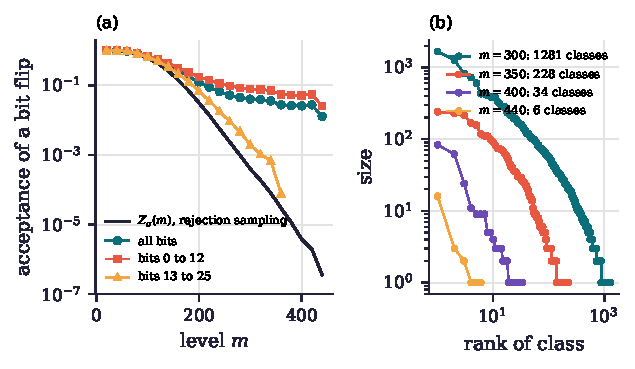
\includegraphics[width=\textwidth]{figures/ch10c_acceptance.pdf}
\caption{Coalescence or independence. (a) Acceptance rate of a single bit flip
inside the level set $\{\sigma_\infty>m\}\cap[2,2^{26})$, for all bits, for the
low bits and for the high bits, against the acceptance rate $Z_\sigma(m)$ of rejection sampling. Low
bit flips coalesce and keep accepting; high bit flips rarely coalesce and
stop. (b) Sizes of the coalescence classes of the level sets at
$m=300,350,400,440$, ranked. The $257$ integers above $400$ form $34$ classes,
$83$ of them in the largest; the $24$ above $440$ form six.}
\label{fig:ch10b:acceptance}
\end{figure}

At the deepest levels the confinement is exact in the data.
\Cref{tab:ch10b:clusters} decomposes each level set into coalescence classes,
two integers being in the same class if their orbits meet at a point whose
remaining stopping time is at least $m-100$ (the meeting point may lie above the
box, and usually does). The $26\,708$ integers above $300$
fall into $1\,281$ classes, the largest with $1\,659$ members; the $257$ above
$400$ fall into $34$, with $83$ in the largest; the $24$ above $440$ fall into
six. And of the $172$ accepted single bit flips among the integers above $400$ (the $86$ pairs that differ in one bit, each counted in both directions), all $172$ stay in the same class.
Not one crosses between classes, as the heuristic suggests, since a
crossing would be an independent orbit of length above $400$ found by a single
proposal.
At $m=300$ and $m=350$ some accepted flips do cross, $1\,112$ of $27\,896$ and $22$ of $2\,848$, that is $1.6\times10^{-3}$ and $2.5\times10^{-4}$ of all proposals, against the values $9.8\times10^{-4}$ and $1.3\times10^{-4}$ of $e^{DB}Z_\sigma(m)$ in the heuristic.

\begin{table}[t]
\centering\small
\caption{Coalescence classes of the level sets $\{\sigma_\infty>m\}$ on
$[2,2^{26})$, two integers being equivalent if their orbits merge no later than the point where the remaining stopping time equals $m-100$. The last two columns count the accepted single bit flips, that is the ordered pairs of integers in the level set that differ in one bit, and how many of them stay in the same class.}
\label{tab:ch10b:clusters}
\begin{tabular}{@{}rrrrrr@{}}
\toprule
$m$ & integers & classes & largest & accepted flips & same class \\
\midrule
$300$ & $26\,708$ & $1\,281$ & $1\,659$ & $27\,896$ & $26\,784$ \\
$350$ & $3\,432$ & $228$ & $240$ & $2\,848$ & $2\,826$ \\
$400$ & $257$ & $34$ & $83$ & $172$ & $172$ \\
$440$ & $24$ & $6$ & $16$ & $8$ & $8$ \\
\bottomrule
\end{tabular}
\end{table}

This is the right description of the far side of the horizon. A deep level set
is not a sparse set of unrelated integers; it is a small number of trees, each
the set of all tributaries of one slow orbit, and a local sampler stays in the tree it starts in, leaving it only rarely, at a rate per proposal of the order of the acceptance rate of rejection sampling. Inside the tree it is confined further, to the few members within a few bit flips of its current point: the $86$ pairs that differ in one bit join the $257$ integers above $400$ into at least $171$ separate pieces, and each stalled stage of split sampling reported below visited between one and twenty three distinct integers. The number of trees is what shrinks with
the depth, not the acceptance rate: $34$ at $400$, six at $440$. A level set
sampler therefore does not degrade into rejection sampling. It does something
more specific. It stays in the tree it starts in, and in fact among a handful of its members, and it
cannot climb above the maximum of $\sigma_\infty$ on that tree, because every
integer it can reach shares the tail of the same orbit. Its depth is bounded
by the deepest tree its initial population happens to contain, and new trees
are found only by independent draws from the prior or by the rare crossing proposals, at about the acceptance rate of rejection sampling.

How the trees multiply with the size of the box is shown in
\cref{tab:ch10b:trees}, which repeats the decomposition on $[2,2^B)$ for
$B=22,24,26$. At a fixed level and over $22\le B\le26$ the number of trees grows with $B$ at a rate
between $2^{B}$ and $2^{1.4B}$, faster at deeper levels, while the mean tree
size grows roughly like $2^{0.4B}$ and, at fixed $B$, falls steadily with the depth,
from $208$ at $m=200$ to $7.6$ at $m=400$ for $B=26$.
These are local exponents: at a fixed level the number of trees is bounded in $B$, since each tree has its own root, an integer with $\sigma_\infty=m-100$, and all such integers are at most $2^{m-100}$, because a step of $T$ at most halves.
A tree is the set of
predecessors below $2^B$ of one point $x$ at remaining depth $m-100$ that lie
more than a hundred steps above $x$, so its size is a count on the inverse tree
of \cref{chap:difference} and the number of trees is the number of such points
$x$ that are reached from the box by an orbit segment of more than a hundred steps. At the deeper levels the root $x$ usually lies above the box: at $m=400$ the roots of the two largest trees are
$146\,053\,012$ and $1\,330\,038\,578$, well beyond $2^{26}$, because a slow
orbit of a box integer climbs out of the box long before its remaining stopping
time falls to $300$. The trees are also mostly tributary: of the $83$ members
of the largest tree at $m=400$ only $14$ lie on the orbit of its deepest member,
the rest being integers whose orbits join that orbit later.

The deepest member of a tree is sometimes a delay record of \cref{chap:intro} (for $2$ of the $34$ trees at $m=400$), but
the correspondence is loose. At $m=400$ three of the $34$ trees contain a
record, including the two largest, whose deepest members are $55\,285\,737$
($\sigma_\infty=446$) and the record $36\,791\,535$ ($466$); the overall
record $63\,728\,127$, with $\sigma_\infty=592$, is a tree of one member at
$m=440$, because its orbit leaves the box at once and nothing below $2^{26}$
joins it in time. The records are the deepest trunks; the large trees are the
trunks that stay low enough, for long enough, to collect tributaries. A naive
model of tree size, in which each backward path of $d$ steps with $j$ odd
steps from $x$ exists with the integrality probability $3^{-j}$, predicts
fewer than four members for every root at $m\ge350$ and is wrong by three orders of magnitude or more: the median ratio of observed to predicted size is about $1.6\times10^3$ at $m=350$ and $10^4$ at $m=400$, where the largest tree has $83$ members against a prediction of $0.012$. Conditioned on being reached from the box by a slow orbit, a
root is reached by many, and the conditioning is the likely explanation. We do not
have a model that predicts either the number of trees or their sizes, and we
record the question as project P9 of \cref{chap:open}.

\begin{table}[t]
\centering\small
\caption{Trees of slow integers on $[2,2^B)$: the number of integers with
$\sigma_\infty>m$, the number of coalescence classes, and their mean and
largest size, for three box sizes.}
\label{tab:ch10b:trees}
\setlength{\tabcolsep}{4pt}\begin{tabular}{@{}rrrrrr@{}}
\toprule
$B$ & $m$ & integers & trees & mean size & largest \\
\midrule
$22$ & $200$ & $36\,482$ & $647$ & $56.4$ & $2\,224$ \\
$22$ & $250$ & $2\,558$ & $204$ & $12.5$ & $198$ \\
$22$ & $300$ & $201$ & $29$ & $6.9$ & $65$ \\
$24$ & $200$ & $291\,361$ & $2\,539$ & $114.8$ & $15\,153$ \\
$24$ & $250$ & $28\,429$ & $1\,047$ & $27.2$ & $1\,320$ \\
$24$ & $300$ & $2\,610$ & $184$ & $14.2$ & $381$ \\
$24$ & $350$ & $259$ & $33$ & $7.8$ & $42$ \\
$26$ & $200$ & $2\,125\,551$ & $10\,235$ & $207.7$ & $110\,856$ \\
$26$ & $250$ & $253\,975$ & $5\,682$ & $44.7$ & $8\,424$ \\
$26$ & $300$ & $26\,708$ & $1\,281$ & $20.8$ & $1\,659$ \\
$26$ & $350$ & $3\,432$ & $228$ & $15.1$ & $240$ \\
$26$ & $400$ & $257$ & $34$ & $7.6$ & $83$ \\
\bottomrule
\end{tabular}
\end{table}

\section{The three samplers against the census}

We tested the three samplers on the prior uniform on $[2,2^{26})$, with energy
the total stopping time of $T$ and the exact $Z_\sigma$ from the census of
\cref{chap:stochastic} (the maximum is $\sigma_\infty=592$, at
$n=63\,728\,127$). Each sampler had a budget of at most $2\times10^5$ energy evaluations per run, and the level set samplers used a kernel step that flips one to three random bits. Naive sampling used exactly $2\times10^5$ independent draws; nested sampling ran $200$ live points for $1600$ iterations with $120$ kernel steps per replacement ($192\,200$ evaluations); split sampling took $1200$ samples per stage, ten kernel steps apart, with $\rho=e^{-1}$, and stopped at the first stage that found no sample above its quantile (between $105\,300$ and $176\,510$ evaluations); and the vertical likelihood sampler ran $12\,000$ sweeps of $16$ kernel steps ($192\,000$ evaluations) with a floor $\eta=10^{-7}$ and the running estimate of $Z$ refreshed every $2000$ sweeps.
\Cref{tab:ch10b:mc} reports the medians of six independent runs.

\begin{table}[t]
\centering\small
\caption{Estimates of $Z_\sigma(m)=\Prob\{\sigma_\infty>m\}$ on $[2,2^{26})$,
medians of six runs at a budget of at most $2\times10^5$ energy evaluations each. The
exact values are from the census. From $m=400$ on, nested and split sampling report the prior mass of their last level, the vertical likelihood estimate is zero in four of the six runs at $m=400$, and so in the median, and in all six at $m=450$ and $500$, and naive sampling sees at most two integers above $400$ in a run and none above $450$.}
\label{tab:ch10b:mc}
\setlength{\tabcolsep}{4pt}\begin{tabular}{@{}rlllll@{}}
\toprule
$m$ & exact & naive & nested & split & vertical \\
\midrule
$100$ & $6.13\times10^{-1}$ & $6.13\times10^{-1}$ & $6.47\times10^{-1}$ & $4.57\times10^{-1}$ & $5.21\times10^{-1}$ \\
$200$ & $3.17\times10^{-2}$ & $3.18\times10^{-2}$ & $3.37\times10^{-2}$ & $3.25\times10^{-2}$ & $1.25\times10^{-2}$ \\
$300$ & $3.98\times10^{-4}$ & $3.75\times10^{-4}$ & $4.56\times10^{-4}$ & $1.94\times10^{-4}$ & $3.85\times10^{-5}$ \\
$400$ & $3.83\times10^{-6}$ & $5.0\times10^{-6}$ & $3.35\times10^{-4}$ & $2.54\times10^{-5}$ & $0$ \\
$450$ & $1.04\times10^{-7}$ & $0$ & $3.35\times10^{-4}$ & $2.54\times10^{-5}$ & $0$ \\
$500$ & $1.49\times10^{-8}$ & $0$ & $3.35\times10^{-4}$ & $2.54\times10^{-5}$ & $0$ \\
\bottomrule
\end{tabular}
\end{table}

\begin{figure}[t]
\centering
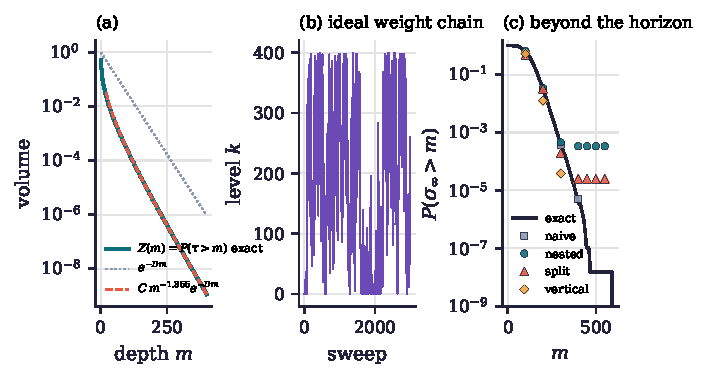
\includegraphics[width=\textwidth]{figures/ch10c_montecarlo.pdf}
\caption{Simulation on both sides of the horizon. (a) The exact staircase
$Z_\tau(m)=\Prob\{\tau>m\}$ under Haar measure, against $e^{-Dm}$ and the fit
$Cm^{-1.355}e^{-Dm}$ over $100\le m\le400$. (b) The level of the perfect split sampler of
\cref{thm:ch10b:perfect} at depth $K=400$, over the first $3000$ of twenty thousand sweeps: a free random walk on
the stopping levels up to the depth $400$ of the run, where the prior mass is
$1.2\times10^{-9}$. (c) The same methods applied to the total stopping time on
$[2,2^{26})$: exact $Z_\sigma$ against the medians of naive, nested, split and
vertical likelihood estimates. Naive and nested sampling track the truth to depth $300$, split sampling within a factor of about two there, and the vertical likelihood sampler only to depth $200$, within a factor of $2.5$; beyond depth $300$ the level set estimates stop changing or vanish.}
\label{fig:ch10b:montecarlo}
\end{figure}

Up to $m=200$ all four estimates agree with the truth to within a factor of about two and a half.
At $m=300$, where $Z_\sigma$ is $4\times10^{-4}$ and the budget contains some eighty naive hits, naive and nested sampling are within $15\%$ of the truth and split sampling is low by a factor of about two, while the vertical likelihood estimate is already low by a factor of ten; the level set methods bring nothing here, because the levels are still cheap.
Beyond $m=300$ the level set samplers stop, for two different reasons.
Split sampling stopped in every run at a level between $303$ and $338$, in a stage whose chain never left one coalescence class: it visited between one and twenty three distinct integers, all with the same total stopping time, so that no sample lay above the quantile. That is the confinement of the tree picture, and the estimate beyond that level is the product of the stage fractions found so far.
Nested sampling stopped for want of budget: its $1600$ iterations shrink the prior volume to $e^{-1600/200}=3.35\times10^{-4}$, which its six runs reached at thresholds between $297$ and $322$, and its estimate of $Z_\sigma(m)$ for every $m$ above the last threshold is that final volume.
At the end its live points occupied between $12$ and $36$ of the $573$ to $1\,331$ coalescence classes at the final threshold, and in every run some occupied class had a member above $400$, the deepest lying between $419$ and $466$; reaching $m=400$, where $Z_\sigma=e^{-12.5}$, would have needed about $2500$ iterations, more than the budget allows, so the table does not show whether nested sampling would be trapped in its trees.
The vertical likelihood chain visited energies up to between $381$ and $446$ in the six runs, but four runs never went above $400$, so its median estimate there is zero.
Naive sampling by contrast sees about one integer above $400$ per run, since $2\times10^5\times3.8\times10^{-6}\approx0.8$ (the six runs see $2$, $1$, $1$, $0$, $2$ and $0$), and is the best of the four there, because an independent draw is not confined to a tree.
The compression factors that make nested and split sampling
polynomial in the depth presuppose that the constrained kernel delivers an
independent point of the level set; in the stage where split sampling stopped it delivered another tributary of the same orbit, or the same integer again.

The expected value that \eqref{eq:ch10b:cake} delivers in this setting is the
mean total stopping time on the box, $\E[\sigma_\infty]=116.9$ at $B=26$, and
the Boltzmann evidence $\E[e^{\beta\sigma_\infty}]$, which nested sampling
(a separate run with $400$ live points, $6000$ iterations and $20$ single bit flips per replacement, script \texttt{ch10b\_nested.py}) estimates at $\beta=0.02$ as $16.2$ against the exact $15.4$: good enough, and
irrelevant, because both are averages over the integers that do reach $1$.

\section{What simulation can and cannot decide}

We can now state the verdict with some precision.

\begin{enumerate}[label=(\roman*),leftmargin=2em]
\item The conjecture is a universal statement: no positive integer lies in every set of the nest $\{\sigma_\infty>m\}$. A sampler explores the nest at finite depth.
  Under Haar measure this nest carries no signal at any depth: every $\{\sigma_\infty>m\}$ has measure one by \cref{prop:ch10b:horizons}(ii), and so does the limit $\{\sigma_\infty=\infty\}$, which contains $0$ and every negative integer; the positive integers in the limit form a countable set, hence a Haar null set, and the conjecture says that there are none.
  The residue nest $\{\tau>m\}$, which a sampler can navigate, decreases to the set $E=\{\tau=\infty\}$, which has Haar measure zero by \cref{prop:ch10b:horizons}(i), contains $-1$, $-5$ and $-17$, and contains no integer $n\ge2$ if the conjecture is true (\cref{prop:ch10b:residue}(iii)). Either way the target is a null set.
  No Monte Carlo method
  samples a null set, and a method that is polynomial in the depth is
  polynomial in a parameter that must go to infinity.
\item What simulation does in polynomial time is sample and measure the
  exceptional classes at depth $m$: the residues with $\tau>m$, exactly and
  with no Markov chain, by \cref{thm:ch10b:perfect}. These are the classes the
  residue sieve of \cref{sec:ch10b:divergence} enumerates, and the sampler is
  the randomized version of the sieve. Any computation that needs typical
  members of the exceptional classes, for instance to test a candidate
  potential or to seed a search for a certificate, has an exact tool.
\item Beyond the horizon, which is the bit length of the integers being
  sampled, a deep level set is a small number of trees of merged orbits
  (\cref{prop:ch10b:acceptance}, \cref{rem:ch10c:coalescence}, \cref{tab:ch10b:clusters}). A local sampler
  stays among a few members of one tree and leaves the tree only rarely, at about the acceptance rate of rejection sampling, so its depth is essentially the depth of the trees
  its initial population contains, and new trees are found by independent draws or by rare crossings, at about that rate.
  Estimating the number of slow integers below $2^B$ at levels where $Z_\sigma(m)$ is far below the reciprocal of the sampling budget therefore costs what it costs the
  census, and the census is exact.
\item The energy whose level sets a sampler can sample exactly at every depth is a function of a
  finite parity word; the energy the conjecture concerns is not. The gap
  between the two is the integrality gap of \cref{prop:ch10b:residue} once
  more: a sampler moves through residue classes, and the conjecture is about
  integers.
\end{enumerate}

So the answer to the question that opened this chapter is no. Simulation does
not decide the conjecture in polynomial time, or in any time, and the
obstruction is not one of efficiency but of what the level sets are. What
simulation offers, and this is worth having, is three things: the perfect
sampler of \cref{thm:ch10b:perfect} and the hazard description of the staircase,
which make the exceptional set at every finite depth a computable and
samplable object; the tree decomposition of the deep level sets, which says
that, in the boxes we computed, the slow integers are a small number of long orbits
together with their tributaries; and a heuristic account, borne out by the census, of why the one method
that moves freely between trees, independent sampling, is the one that costs
$1/Z_\sigma(m)$.

\section*{Notes}

Nested sampling\index{nested sampling} is Skilling's~\cite{skilling2006};
the vertical likelihood\index{vertical likelihood} view of it, and the weighted slice sampler that
places several level set methods in one scheme, are from Polson and Scott~\cite{polsonscott2015};
split sampling\index{split sampling}, with its Rao Blackwellized volume curve and its correspondences with the product estimator and with nested sampling, is from Birge, Chang and Polson~\cite{birge2013}; the slice sampler
itself is Neal's\index{Neal, R. M.}~\cite{neal2003}.
The weight $W=1/Z$ makes the level histogram flat in $\log(1/Z)$, while the flat energy histogram that the Wang\index{Wang, F.} and Landau\index{Landau, D. P.}\index{Wang and Landau algorithm} algorithm~\cite{wanglandau2001} aims at comes from weighting by the inverse density of states~\cite[Section~2]{polsonscott2015}.
The perfect sampler of \cref{thm:ch10b:perfect} is ours as a sampler, but its backward step is the classical recursive method of uniform generation from counts of Nijenhuis\index{Nijenhuis, A.} and Wilf\index{Wilf, H. S.}~\cite{nijenhuis1978}; the proposition on the two energies, the
coalescence heuristic and the tree decomposition of the deep level sets are
ours; the merging of consecutive integers under the map is classical (Garner\index{Garner, L. E.}~\cite{garner1985} used it to show that infinitely many pairs of consecutive integers have the same total stopping time) and is
the source of the confluences in every picture of the Collatz graph.

\section*{Exercises}

\begin{exercise}
Implement the backward sampler of \cref{thm:ch10b:perfect} and draw ten
residues modulo $2^{200}$ with $\tau>200$. Verify directly that each has more
than $200/\lt$ ones among its first $200$ parities, and estimate from a
thousand draws the mean number of ones at depth $200$. Compare with the
conditional law $j\mapsto N_{200}(j)/\sum_{j'}N_{200}(j')$.
\end{exercise}

\begin{exercise}
In the Bernoulli model of \cref{chap:stochastic}, show that the tail of the total stopping time has the same
exponential rate $D=\log2-H(1/\lt)$ as $\Prob\{\tau>m\}$, and explain why, in the model with starting points uniform on $[2,2^B)$, the box changes the prefactor but not the rate for $m\gg B$. (For the census itself $Z_\sigma(m)=0$ for $m\ge592$, the largest total stopping time in the box for $B=26$.)
\end{exercise}
